%---------------------------------------------------------------------------%
%-                                                                         -%
%-                           LaTeX Template                                -%
%-                                                                         -%
%---------------------------------------------------------------------------%
%- Copyright (C) Huangrui Mo <huangrui.mo@gmail.com> 
%- This is free software: you can redistribute it and/or modify it
%- under the terms of the GNU General Public License as published by
%- the Free Software Foundation, either version 3 of the License, or
%- (at your option) any later version.
%---------------------------------------------------------------------------%
%->> Document class declaration
%---------------------------------------------------------------------------%
\documentclass[doublesided]{Style/ucasthesis}%
%- Multiple optional arguments:
%- [<singlesided|doublesided|printcopy>]% set one or two sided eprint or print
%- [draftversion]% show draft version information
%- [fontset=<fandol|...>]% specify font set to replace automatic detection
%- [scheme=plain]% thesis writing of international students
%- [standard options for ctex book class: draft|paper size|font size|...]%
%---------------------------------------------------------------------------%
%->> Document settings
%---------------------------------------------------------------------------%
\usepackage[authoryear,myhdr,list]{Style/artratex}% document settings
%- usage: \usepackage[option1,option2,...,optionN]{artratex}
%- Multiple optional arguments:
%- [bibtex|biber]% set bibliography processor and package
%- [<numbers|super|authoryear|alpha>]% set citation and reference style
%- <numbers>: textual: Jones [1]; parenthetical: [1]
%- <super>: textual: Jones superscript [1]; parenthetical: superscript [1]
%- <authoryear>: textual: Jones (1995); parenthetical: (Jones, 1995)
%- <alpha>: textual: not available; parenthetical: [Jon95]
%- [geometry]% reconfigure page layout via geometry package
%- [lscape]% provide landscape layout environment
%- [myhdr]% enable header and footer via fancyhdr package
%- [color]% provide color support via xcolor package
%- [background]% enable page background
%- [tikz]% provide complex diagrams via tikz package
%- [table]% provide complex tables via ctable package
%- [list]% provide enhanced list environments for algorithm and coding
%- [math]% enable some extra math packages
\usepackage{Style/artracom}% user defined commands

%%%%%%%%%%%%%%
\usepackage{fancyvrb}
\usepackage{hologo}

% \setlength{\hfuzz}{3pt}
% \ctexset{linestretch = 2\ccwd}
% \setlength{\bibitemsep}{3bp}
% \renewcommand*{\bibfont}{\zihao{5}\linespread{1.27}\selectfont}

\hypersetup{colorlinks = true, allcolors = blue}
\newcommand{\myemph}[1]{\emph{\textcolor{red}{#1}}}
\newcommand{\unemph}[1]{\textup{\textcolor{black}{#1}}}
\newcommand{\docversion}{v1.7.4}

\usepackage{longtable,booktabs}

\usepackage{amssymb,amsmath}
%\usepackage{natbib}
%\bibliographystyle{apalike}
\newcommand{\VerbBar}{|}
\newcommand{\VERB}{\Verb[commandchars=\\\{\}]}
\DefineVerbatimEnvironment{Highlighting}{Verbatim}{commandchars=\\\{\}}
% Add ',fontsize=\small' for more characters per line
\usepackage{framed}
\definecolor{shadecolor}{RGB}{248,248,248}
\newenvironment{Shaded}{\begin{snugshade}}{\end{snugshade}}
\newcommand{\KeywordTok}[1]{\textcolor[rgb]{0.13,0.29,0.53}{\textbf{{#1}}}}
\newcommand{\DataTypeTok}[1]{\textcolor[rgb]{0.13,0.29,0.53}{{#1}}}
\newcommand{\DecValTok}[1]{\textcolor[rgb]{0.00,0.00,0.81}{{#1}}}
\newcommand{\BaseNTok}[1]{\textcolor[rgb]{0.00,0.00,0.81}{{#1}}}
\newcommand{\FloatTok}[1]{\textcolor[rgb]{0.00,0.00,0.81}{{#1}}}
\newcommand{\ConstantTok}[1]{\textcolor[rgb]{0.00,0.00,0.00}{{#1}}}
\newcommand{\CharTok}[1]{\textcolor[rgb]{0.31,0.60,0.02}{{#1}}}
\newcommand{\SpecialCharTok}[1]{\textcolor[rgb]{0.00,0.00,0.00}{{#1}}}
\newcommand{\StringTok}[1]{\textcolor[rgb]{0.31,0.60,0.02}{{#1}}}
\newcommand{\VerbatimStringTok}[1]{\textcolor[rgb]{0.31,0.60,0.02}{{#1}}}
\newcommand{\SpecialStringTok}[1]{\textcolor[rgb]{0.31,0.60,0.02}{{#1}}}
\newcommand{\ImportTok}[1]{{#1}}
\newcommand{\CommentTok}[1]{\textcolor[rgb]{0.56,0.35,0.01}{\textit{{#1}}}}
\newcommand{\DocumentationTok}[1]{\textcolor[rgb]{0.56,0.35,0.01}{\textbf{\textit{{#1}}}}}
\newcommand{\AnnotationTok}[1]{\textcolor[rgb]{0.56,0.35,0.01}{\textbf{\textit{{#1}}}}}
\newcommand{\CommentVarTok}[1]{\textcolor[rgb]{0.56,0.35,0.01}{\textbf{\textit{{#1}}}}}
\newcommand{\OtherTok}[1]{\textcolor[rgb]{0.56,0.35,0.01}{{#1}}}
\newcommand{\FunctionTok}[1]{\textcolor[rgb]{0.00,0.00,0.00}{{#1}}}
\newcommand{\VariableTok}[1]{\textcolor[rgb]{0.00,0.00,0.00}{{#1}}}
\newcommand{\ControlFlowTok}[1]{\textcolor[rgb]{0.13,0.29,0.53}{\textbf{{#1}}}}
\newcommand{\OperatorTok}[1]{\textcolor[rgb]{0.81,0.36,0.00}{\textbf{{#1}}}}
\newcommand{\BuiltInTok}[1]{{#1}}
\newcommand{\ExtensionTok}[1]{{#1}}
\newcommand{\PreprocessorTok}[1]{\textcolor[rgb]{0.56,0.35,0.01}{\textit{{#1}}}}
\newcommand{\AttributeTok}[1]{\textcolor[rgb]{0.77,0.63,0.00}{{#1}}}
\newcommand{\RegionMarkerTok}[1]{{#1}}
\newcommand{\InformationTok}[1]{\textcolor[rgb]{0.56,0.35,0.01}{\textbf{\textit{{#1}}}}}
\newcommand{\WarningTok}[1]{\textcolor[rgb]{0.56,0.35,0.01}{\textbf{\textit{{#1}}}}}
\newcommand{\AlertTok}[1]{\textcolor[rgb]{0.94,0.16,0.16}{{#1}}}
\newcommand{\ErrorTok}[1]{\textcolor[rgb]{0.64,0.00,0.00}{\textbf{{#1}}}}
\newcommand{\NormalTok}[1]{{#1}}
%%%%%%%%%%%%%%


%---------------------------------------------------------------------------%
%->> Document inclusion
%---------------------------------------------------------------------------%
%\includeonly{Tex/Chap_1,...,Tex/Chap_N}% selected files compilation
%---------------------------------------------------------------------------%
%->> Document content
%---------------------------------------------------------------------------%
\begin{document}
%-
%-> Frontmatter: title page, abstract, content list, symbol list, preface
%-
\frontmatter% initialize the environment

%---------------------------------------------------------------------------%
%->> 封面信息及生成
%---------------------------------------------------------------------------%
%-
%-> 中文封面信息
%-
\confidential{}% 密级:只有涉密论文才填写
\schoollogo{scale=0.095}{ucas_logo}% 校徽
\title{中国科学院大学学位论文 bookdown 模板}% 论文中文题目
\author{author}% 论文作者
\advisor{谷哥教授}% 指导教师:姓名 专业技术职务 工作单位
\advisorsec{}% 指导老师附加信息 或 第二指导老师信息
\degree{硕士}% 学位:学士、硕士、博士
\degreetype{理学}% 学位类别:理学、工学、工程、医学等
\major{论文排版}% 二级学科专业名称
\institute{R 语言学院}% 院系名称
\chinesedate{2018 年 9 月}% 毕业日期:夏季为6月、冬季为12月
%-
%-> 英文封面信息
%-
\englishtitle{R bookdownplus}% 论文英文题目
\englishauthor{dapeng}% 论文作者
\englishadvisor{Supervisor: Prof.Google}% 指导教师
\englishdegree{Master}% 学位:Bachelor, Master, Doctor。封面格式将根据英文学位名称自动切换,请确保拼写准确无误
\englishdegreetype{Natural Science}% 学位类别:Philosophy, Natural Science, Engineering, Economics, Agriculture 等
\englishthesistype{thesis}% 论文类型: thesis, dissertation
\englishmajor{Typesetting}% 二级学科专业名称
\englishinstitute{College of R}% 院系名称
\englishdate{September, 2018}% 毕业日期:夏季为June、冬季为December
%-
%-> 生成封面
%-
\maketitle% 生成中文封面
\makeenglishtitle% 生成英文封面
%-
%-> 作者声明
%-
\makedeclaration% 生成声明页
%-
%-> 中文摘要
%-
\chapter*{摘\quad 要}\chaptermark{摘\quad 要}% 摘要标题
\setcounter{page}{1}% 开始页码
\pagenumbering{Roman}% 页码符号

这里写中文摘要。啊不可挡家真的好。

\keywords{排版,文档类}% 中文关键词
%-
%-> 英文摘要
%-
\chapter*{Abstract}\chaptermark{Abstract}% 摘要标题

Abstract in English. R bookdownplus is amazing.

\englishkeywords{\hologo{LaTeX2e}, \CTeX{}, bookdown}% 英文关键词
%---------------------------------------------------------------------------%



{% content list region
\linespread{1.2}% local line space
%\intotoc{\contentsname}% add link to contents table and bookmark
\tableofcontents% contents catalog
%\intotoc{\listfigurename}% add link to contents table and bookmark
\listoffigures% figures catalog
%\intotoc{\listtablename}% add link to contents table and bookmark
\listoftables% tables catalog
}
\chapter*{符号列表}
\chaptermark{符号列表}

\section*{字符}
\nomenclatureitem[\textbf{Unit}]{\textbf{Symbol}}{\textbf{Description}}
\nomenclatureitem[$\Unit{m^{2} \cdot s^{-2} \cdot K^{-1}}$]{$R$}{the gas constant}
\nomenclatureitem[$\Unit{m^{2} \cdot s^{-2} \cdot K^{-1}}$]{$C_v$}{specific heat capacity at constant volume}
\nomenclatureitem[$\Unit{m^{2} \cdot s^{-2} \cdot K^{-1}}$]{$C_p$}{specific heat capacity at constant pressure}
\nomenclatureitem[$\Unit{m^{2} \cdot s^{-2}}$]{$E$}{specific total energy}
\nomenclatureitem[$\Unit{m^{2} \cdot s^{-2}}$]{$e$}{specific internal energy}
\nomenclatureitem[$\Unit{m^{2} \cdot s^{-2}}$]{$h_T$}{specific total enthalpy}
\nomenclatureitem[$\Unit{m^{2} \cdot s^{-2}}$]{$h$}{specific enthalpy}
\nomenclatureitem[$\Unit{kg \cdot m \cdot s^{-3} \cdot K^{-1}}$]{$k$}{thermal conductivity}
\nomenclatureitem[$\Unit{kg \cdot m^{-1} \cdot s^{-2}}$]{$S_{ij}$}{deviatoric stress tensor}
\nomenclatureitem[$\Unit{kg \cdot m^{-1} \cdot s^{-2}}$]{$\tau_{ij}$}{viscous stress tensor}
\nomenclatureitem[$\Unit{1}$]{$\delta_{ij}$}{Kronecker tensor}
\nomenclatureitem[$\Unit{1}$]{$I_{ij}$}{identity tensor}

\section*{算子}
\nomenclatureitem{\textbf{Symbol}}{\textbf{Description}}
\nomenclatureitem{$\Delta$}{difference}
\nomenclatureitem{$\nabla$}{gradient operator}
\nomenclatureitem{$\delta^{\pm}$}{upwind-biased interpolation scheme}

\section*{缩写}
\nomenclatureitem{CFD}{Computational Fluid Dynamics}
\nomenclatureitem{CFL}{Courant-Friedrichs-Lewy}
\nomenclatureitem{EOS}{Equation of State}
\nomenclatureitem{JWL}{Jones-Wilkins-Lee}
\nomenclatureitem{WENO}{Weighted Essentially Non-oscillatory}
\nomenclatureitem{ZND}{Zel'dovich-von Neumann-Doering}

% list of symbols, preface content
%-
%-> Mainmatter
%-
\mainmatter% initialize the environment
\mainmatter

\hypertarget{section}{%
\chapter{引言}\label{section}}

很高兴地宣布,我的 R 语言扩展包 `bookdownplus' (Zhao \protect\hyperlink{ref-R-bookdownplus}{2017}) 在 CRAN 正式发布了。

bookdownplus 是对 bookdown 包 (Xie \protect\hyperlink{ref-R-bookdown}{2016}) 的增强和简化。bookdown 就好比 Microsoft Word 或 LaTeX,可以用来写文档,而 bookdownplus 提供了很多有用的模板,可以很方便地在 bookdown 平台写期刊论文、学位论文、学术海报、化学分子式、信件、日记、日历、诗集、吉他谱等各种常用文档和书籍。这是功能上的增强(+)。

bookdownplus 使用时只需指定一个模板,给定作者和书名,就可以一键生成模板文件,用户在模板文件里照猫画虎写自己的文字就可以了,不必再花力气上网找模板、设置 YAML 和 LaTeX。这是操作上的简化(-)。

bookdownplus 各个模板的使用方法详见 \href{https://bookdown.org/baydap/bookdownplus}{R bookdownplus Textbook}。这本电子书本身就是用 bookdownplus 生成的,尤其是它的 \href{https://bookdown.org/baydap/bookdownplus/bookdownplus.pdf}{pdf 版本}很美观。此书的源码开放,可以作为使用 bookdownplus写书的示例。

\begin{figure}

{\centering 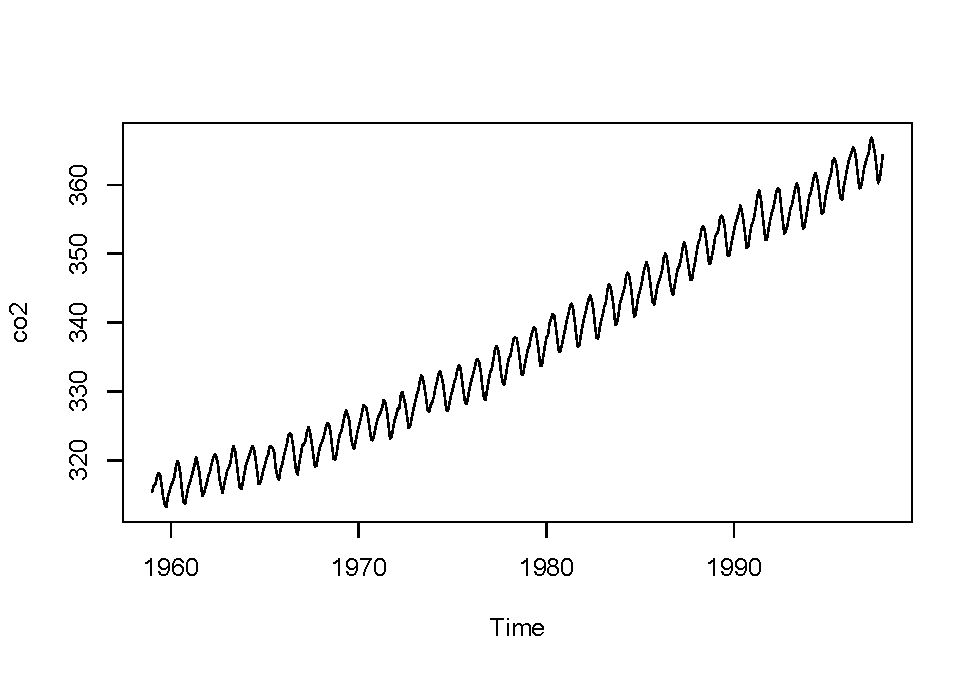
\includegraphics[width=0.8\linewidth]{ucas_zh_files/figure-latex/co2-1} 

}

\caption{用 R 语言画个图试试}\label{fig:co2}
\end{figure}

图 \ref{fig:co2} 是 CO\textsubscript{2} 数据。

表 \ref{tab:tabair} 是空气质量数据。

\begin{Shaded}
\begin{Highlighting}[]
\NormalTok{knitr}\OperatorTok{::}\KeywordTok{kable}\NormalTok{(}\KeywordTok{head}\NormalTok{(airquality), }\DataTypeTok{caption =} \StringTok{'空气质量数据。'}\NormalTok{,}
                   \DataTypeTok{booktabs =} \OtherTok{TRUE}\NormalTok{)}
\end{Highlighting}
\end{Shaded}

\begin{table}[t]

\caption{\label{tab:tabair}空气质量数据。}
\centering
\begin{tabular}{rrrrrr}
\toprule
Ozone & Solar.R & Wind & Temp & Month & Day\\
\midrule
41 & 190 & 7.4 & 67 & 5 & 1\\
36 & 118 & 8.0 & 72 & 5 & 2\\
12 & 149 & 12.6 & 74 & 5 & 3\\
18 & 313 & 11.5 & 62 & 5 & 4\\
NA & NA & 14.3 & 56 & 5 & 5\\
\addlinespace
28 & NA & 14.9 & 66 & 5 & 6\\
\bottomrule
\end{tabular}
\end{table}

\hypertarget{section-1}{%
\chapter{材料与方法}\label{section-1}}

\hypertarget{section-2}{%
\section{准备}\label{section-2}}

在开始前,需要安装 R, RStudio, bookdown,和其他依赖的软件和包(例如 \texttt{Pandoc}, LaTeX, \texttt{rmarkdown}, \texttt{rticle}, \texttt{knitr}等),作为准备。详见 \href{https://bookdown.org/yihui/bookdown/}{bookdown 官方手册}。

\hypertarget{section-3}{%
\section{安装}\label{section-3}}

准备完毕后,就可以安装 bookdownplus 了。可以安装稳定版:

\begin{verbatim}
install.packages("bookdownplus")
\end{verbatim}

或开发版:

\begin{verbatim}
devtools::install_github("pzhaonet/bookdownplus")
\end{verbatim}

\hypertarget{section-4}{%
\section{生成模板文件}\label{section-4}}

接着,在 R 中运行下面的代码:

\begin{verbatim}
bookdownplus::bookdownplus()
\end{verbatim}

这时,在你的工作目录(\texttt{getwd()}),会得到一些模板文件(如 \texttt{index.Rmd},\texttt{body.Rmd}, \texttt{bookdownplus.Rproj}) 和文件夹。

\hypertarget{section-5}{%
\section{编译成书}\label{section-5}}

用 RStudio 打开 \texttt{bookdownplus.Rproj}文件,然后按 \texttt{ctrl+shift+b},Duang!你就得到模板书 \texttt{*.pdf}了!保存在 \texttt{\_book/} 文件夹里。

\hypertarget{section-6}{%
\section{你的文字}\label{section-6}}

在 \texttt{index.Rmd} 和 \texttt{body.Rmd} 里写你自己的文字,享受写书的快乐吧!自古皆死,不朽者文。

\hypertarget{section-7}{%
\section{更多输出格式}\label{section-7}}

模板默认生成的书是pdf格式。`bookdownplus' 从 1.0.3 开始,可以很方便地输出更多格式,包括国内最常见的 'word'格式,网页'html'格式和电子书'epub'格式,只需运行:

\begin{Shaded}
\begin{Highlighting}[]
\NormalTok{bookdownplus}\OperatorTok{::}\KeywordTok{bookdownplus}\NormalTok{(}\DataTypeTok{template =} \StringTok{'article'}\NormalTok{, }
    \DataTypeTok{more_output =} \KeywordTok{c}\NormalTok{(}\StringTok{'html'}\NormalTok{, }\StringTok{'word'}\NormalTok{, }\StringTok{'epub'}\NormalTok{))}
\end{Highlighting}
\end{Shaded}

就可以在 \texttt{\_book/} 文件夹里看到这些文件了。

网页格式可以极其方便地免费发布到 \href{https://bookdown.org}{bookdown.org},只需运行:

\begin{verbatim}
bookdown::publish_book()
\end{verbatim}

这里是 bookdown 书籍的大本营。

\hypertarget{section-8}{%
\section{更多建议}\label{section-8}}

我开发的另外两个 R 包可以配合 `bookdown' 使用:

\begin{itemize}
\item
  mindr,可以从 markdown 或 R markdown 格式的书稿中提取纲要,并且生成思维导图。
\item
  pinyin,可以为书稿的章节标题自动生成\href{https://bookdown.org/yihui/bookdown/cross-references.html}{`\{\#ID\}'}。如果标题里含有汉字,就会自动转换成拼音。
\end{itemize}

具体用法见他们的帮助信息。这两个包已经在 CRAN正式发布,安装命令是:

\begin{verbatim}
install.packages('mindr')
install.packages('pinyin')`.
\end{verbatim}

祝你玩得愉快!

\hypertarget{results}{%
\chapter{结果与讨论}\label{results}}

结了个果。

\hypertarget{conclusion}{%
\chapter{结论}\label{conclusion}}

盖棺定论。

\appendix

\hypertarget{section-9}{%
\chapter{定理推倒}\label{section-9}}

\raggedbottom

\hypertarget{a-}{%
\section{定理 A 的推倒}\label{a-}}

\flushbottom

\backmatter

\hypertarget{section-10}{%
\chapter{作者简历及攻读学位期间发表的学术论文与研究成果}\label{section-10}}

本科生无需此部分。

\hypertarget{section-11}{%
\chapter{致谢}\label{section-11}}

本模板源自 mohuangrui/ucasthesis \LaTeX\{\} 模板\footnote{\url{https://gitlab.com/mohuangrui/ucasthesis}}。感谢!

\hypertarget{section-12}{%
\chapter{参考文献}\label{section-12}}

\bibliography{bib/bib}

\hypertarget{refs}{}
\leavevmode\hypertarget{ref-R-bookdown}{}%
Xie, Yihui. 2016. \emph{Bookdown: Authoring Books and Technical Documents with R Markdown}. Boca Raton, Florida: Chapman; Hall/CRC. \url{https://github.com/rstudio/bookdown}.

\leavevmode\hypertarget{ref-R-bookdownplus}{}%
Zhao, Peng. 2017. \emph{Bookdownplus: Generate Varied Books and Documents with R 'Bookdown' Package}. \url{https://CRAN.R-project.org/package=bookdownplus}.

\end{document}
%---------------------------------------------------------------------------%

